\newcommand*{\BeamerSuffix}{-pres}
\newcommand*{\TransSuffix}{-slides}
% \documentclass{beamerswitch}
\documentclass{beamer}
\setbeamertemplate{navigation symbols}{}

\usepackage{movie15}
\usepackage{amssymb,amsmath}
\usepackage{hyperref}
\usepackage{natbib} 
\usepackage{pgf} 
\usepackage{mathtools}
\usepackage{tikz}
\usepackage{bbm}

\usetheme{Madrid}   % clean, nice.  7/12 page numbers




%\newtheorem{example}{Example}

\newcommand{\expect}{\mathbb{E}}
\newcommand{\variance}{\mathrm{Var}}
\DeclareMathOperator*{\Var}{Var}
\newcommand{\covariance}{\mathrm{Cov}}
\DeclareMathOperator*{\Cov}{Cov}
\newcommand{\prob}{\mathrm{Pr}}
\newcommand{\zeroVec}{\mathbf{0}}
\newcommand{\zeroMat}{\mathbf{0}}
\newcommand{\onesVec}{\mathbf{1}}
\newcommand{\ident}{\mathbf{I}}
\newcommand{\deriv}{\mathrm{d}}
\newcommand{\transpose}{\top}
\newcommand{\costDeriv}[1]{\overline{#1}}
\newcommand{\lossDeriv}{\costDeriv}
\newcommand{\normal}{\mathcal{N}}
\newcommand{\data}{\mathcal{D}}

\newcommand{\dataIdx}{i}
\newcommand{\featIdx}{j}
\newcommand{\dimIdx}{\featIdx}
\newcommand{\paramIdx}{\dimIdx}
\newcommand{\hidIdx}{i}
\newcommand{\classIdx}{k}
\newcommand{\outputIdx}{k}
\newcommand{\classIdxTwo}{\ell}
\newcommand{\featIdxTwo}{j^\prime}
\newcommand{\nfeat}{D}
\newcommand{\ndim}{\nfeat}
\newcommand{\ndata}{N}
\newcommand{\numClasses}{K}
\newcommand{\nout}{\numClasses}
\newcommand{\layerIdx}{\ell}
\newcommand{\numLayers}{L}
\newcommand{\nhid}{M}
\newcommand{\timeIdx}{t}
\newcommand{\ntime}{T}
\newcommand{\contextLen}{K}


\newcommand{\inputIJ}[2]{x^{(#1)}_{#2}}
\newcommand{\inputI}[1]{{\bf x}^{(#1)}}
\newcommand{\inputJ}[1]{x_{#1}}
\newcommand{\inputVec}{{\bf x}}
\newcommand{\inputVecT}[1]{\inputVec^{(#1)}}
\newcommand{\inputVecI}[1]{\inputVec^{(#1)}}
\newcommand{\inputUni}{x}
\newcommand{\inputUniI}[1]{x^{(#1)}}
\newcommand{\inputUniT}[1]{x^{(#1)}}
\newcommand{\inputMatrix}{\mathbf{X}}
\newcommand{\inputMatrixT}[1]{\inputMatrix^{(#1)}}
\newcommand{\targetI}[1]{t^{(#1)}}
\newcommand{\target}{t}
\newcommand{\targetK}[1]{\target_{#1}}
\newcommand{\targets}{\mathbf{t}}
\newcommand{\prediction}{y}
\newcommand{\predictionI}[1]{y^{(#1)}}
\newcommand{\predictionK}[1]{y_{#1}}
\newcommand{\predictionT}[1]{y^{(#1)}}
\newcommand{\predictions}{\mathbf{y}}
\newcommand{\predictionMatrix}{\mathbf{Y}}
\newcommand{\predictionMatrixT}[1]{\predictionMatrix^{(#1)}}
\newcommand{\intermediate}{z}
\newcommand{\intermediateI}[1]{\intermediate^{(#1)}}
\newcommand{\intermediateT}[1]{\intermediate^{(#1)}}
\newcommand{\intermediateK}[1]{\intermediate_{#1}}
\newcommand{\intermediates}{\mathbf{z}}
\newcommand{\intermediateMatrix}{\mathbf{Z}}
\newcommand{\intermediateMatrixT}[1]{\intermediateMatrix^{(#1)}}
\newcommand{\outIntermediate}{r}
\newcommand{\outIntermediateT}[1]{r^{(#1)}}
\newcommand{\outIntermediateK}[1]{\outIntermediate_{#1}}
\newcommand{\outIntermediates}{\mathbf{r}}
\newcommand{\outIntermediateMat}{\mathbf{R}}
\newcommand{\outIntermediateMatrix}{\mathbf{R}}
\newcommand{\outIntermediateMatrixT}[1]{\outIntermediateMatrix^{(#1)}}
\newcommand{\hiddenI}[1]{h_{#1}}
\newcommand{\hiddenT}[1]{h^{(#1)}}
\newcommand{\hiddenIT}[2]{h_{#1}^{(#2)}}
\newcommand{\hiddenLI}[2]{h_{#2}^{(#1)}}
\newcommand{\hiddens}{\mathbf{h}}
\newcommand{\hiddensL}[1]{\hiddens^{(#1)}}
\newcommand{\hiddensT}[1]{\hiddens^{(#1)}}
\newcommand{\hiddenMatrix}{\mathbf{H}}
\newcommand{\hiddenMat}{\hiddenMatrix}
\newcommand{\hiddenMatrixT}[1]{\hiddenMatrix^{(#1)}}
\newcommand{\hiddenMatL}[1]{\hiddenMat^{(#1)}}
\newcommand{\weights}{{\bf w}}
\newcommand{\weightsL}[1]{\weights^{(#1)}}
\newcommand{\weightJ}[1]{w_{#1}}
\newcommand{\weightLIJ}[3]{w^{(#1)}_{#2 #3}}
\newcommand{\weightLKI}[3]{w^{(#1)}_{#2 #3}}
\newcommand{\weightLJ}[2]{w^{(#1)}_{#2}}
\newcommand{\weightKJ}[2]{w_{#1 #2}}
\newcommand{\weightIJ}{\weightKJ}
\newcommand{\weightUni}{w}
\newcommand{\weightMat}{\mathbf{W}}
\newcommand{\weightMatL}[1]{\weightMat^{(#1)}}
\newcommand{\bias}{b}
\newcommand{\biasLI}[2]{\bias^{(#1)}_{#2}}
\newcommand{\biasLK}{\biasLI}
\newcommand{\biasL}[1]{\bias^{(#1)}}
\newcommand{\biasK}[1]{\bias_{#1}}
\newcommand{\biasJ}[1]{\bias_{#1}}
\newcommand{\biases}{\mathbf{b}}
\newcommand{\biasesL}[1]{\biases^{(#1)}}
\newcommand{\threshold}{r}
\newcommand{\featureJ}[1]{\psi_{#1}}
\newcommand{\featureVec}{{\boldsymbol \psi}}
\newcommand{\loss}{\mathcal{L}}
\newcommand{\lossI}[1]{\loss^{(#1)}}
\newcommand{\zeroOneLoss}{\loss_{\rm 0-1}}
\newcommand{\squaredErrorLoss}{\loss_{\rm SE}}
\newcommand{\crossEntropyLoss}{\loss_{\rm CE}}
\newcommand{\logisticCrossEntropyLoss}{\loss_{\rm LCE}}
\newcommand{\softmaxCrossEntropyLoss}{\loss_{\rm SCE}}
\newcommand{\hingeLoss}{\loss_{\rm H}}
\newcommand{\cost}{\mathcal{J}}
\newcommand{\regularizer}{\mathcal{R}}
\newcommand{\lrate}{\alpha}
\newcommand{\learningRate}{\lrate}
\newcommand{\featureMap}{{\boldsymbol \psi}}
\newcommand{\featureMapJ}[1]{\psi_{#1}}
\newcommand{\sigmoid}{\sigma}
\newcommand{\logistic}{\sigmoid}
\newcommand{\activationFunction}{\phi}
\newcommand{\activationFunctionL}[1]{\activationFunction^{(#1)}}
\newcommand{\activationFunctionTwo}{\psi}
\newcommand{\parityFunction}{f_{\rm par}}
\newcommand{\function}{f}
\newcommand{\functionL}[1]{\function^{(#1)}}
\newcommand{\indicatorOf}[1]{\mathbbm{1}_{#1}}
\newcommand{\softmax}{\mathrm{softmax}}
\newcommand{\weightCost}{\lambda}
\newcommand{\genCost}{\mathcal{C}}
\newcommand{\momentumVec}{\mathbf{p}}
\newcommand{\momentumJ}[1]{p_{#1}}
\newcommand{\momentumParam}{\mu}
\newcommand{\genParams}{{\boldsymbol \theta}}
\newcommand{\genParamJ}[1]{\theta_{#1}}
\newcommand{\pData}{p_{\mathcal{D}}}
\newcommand{\bestPrediction}{\prediction_\star}

\newcommand{\obs}{\mathbf{x}}
\newcommand{\obsJ}[1]{x_{#1}}
\newcommand{\obsI}[1]{\obs^{(#1)}}
\newcommand{\pfn}{\mathcal{Z}}
\newcommand{\happiness}{H}
\newcommand{\latents}{\mathbf{z}}

\newcommand{\state}{\mathbf{s}}
\newcommand{\stateT}[1]{\state_{#1}}
\newcommand{\act}{\mathbf{a}}
\newcommand{\actT}[1]{\act_{#1}}
\newcommand{\reward}{r}
\newcommand{\policy}{\pi}
\newcommand{\policyParams}{\boldsymbol{\theta}}
\newcommand{\policyTh}{{\policy_{\policyParams}}}
\newcommand{\MDP}{\mathcal{M}}
\newcommand{\rollout}{\tau}
\newcommand{\expectedReturn}{R}

\newcommand{\discReturn}{G}
\newcommand{\discFactor}{\gamma}
\newcommand{\valueFunc}{V}
\newcommand{\valueFuncPi}{\valueFunc^{\policy}}
\newcommand{\valueFuncPiTh}{\valueFunc^{\policyTh}}
\newcommand{\qFunc}{Q}
\newcommand{\qFuncPi}{\qFunc^{\policy}}
\newcommand{\optPolicy}{\policy^*}
\newcommand{\optQ}{\qFunc^*}

\newcommand{\subspace}{\mathcal{S}}
\newcommand{\projectedInput}{\tilde{\inputVec}}
\newcommand{\projectedInputI}[1]{\projectedInput^{(#1)}}
\newcommand{\codeVec}{\mathbf{z}}
\newcommand{\codeVecI}[1]{\codeVec^{(#1)}}
\newcommand{\dataMean}{\boldsymbol{\mu}}
\newcommand{\dataCov}{\boldsymbol{\Sigma}}
\newcommand{\pcaVec}{\mathbf{u}}

\newcommand{\featureMatrix}{{\boldsymbol \Psi}}
\newcommand{\smootherMatrix}{{\boldsymbol \Omega}}
\newcommand{\smootherMatrixEntry}{\Omega}
\newcommand{\hypothesis}{\mathcal{H}}
\newcommand{\priorMean}{\mathbf{m}}
\newcommand{\priorCov}{\mathbf{S}}
\newcommand{\priorVar}{\eta}
\newcommand{\postMean}{\boldsymbol{\mu}}
\newcommand{\postCov}{\boldsymbol{\Sigma}}
\newcommand{\predMean}{\mu_{\rm pred}}
\newcommand{\predVar}{\sigma^2_{\rm pred}}
\newcommand{\predStd}{\sigma_{\rm pred}}


\newcommand{\given}{\,|\,}
\newcommand{\TODO}[1]{{\color{red} {\bf [[#1]]}}}
\newcommand{\high}[1]{{\color{blue}{#1}}}



\newcommand{\naive}{na{\"\i}ve }





























%\newcommand{\Perp}{\perp\!\!\! \perp}


\newcommand{\Ep}[2]{\ensuremath{E_{#1}\left[{#2}\right]}}
\def\hpY{\mathbf{\bar{\beta}}}

\newcommand{\gaus}[2]{\mathcal{N}\left({#1};\,{#2}\right)}

\newcommand{\comment}[1]{}

\newcommand{\trace}{\text{trace}}
%\newcommand{\det}{\text{det}}

%\newcommand{\bm}{{\mathbf{m}}}
\newcommand{\loss}{{\cal L}}
\newcommand{\cG}{{\cal G}}
\newcommand{\cV}{{\cal V}}
\newcommand{\cE}{{\cal E}}
\newcommand{\cP}{{\cal P}}
\newcommand{\X}{{\cal X}}
\newcommand{\Y}{{\cal Y}}
\newcommand{\bK}{\mathbf{K}}
\newcommand{\bX}{\mathbf{X}}
\newcommand{\bY}{\mathbf{Y}}
\newcommand{\bk}{\mathbf{k}}
\newcommand{\bx}{\mathbf{x}}
\newcommand{\by}{\mathbf{y}}
\newcommand{\bhy}{\hat{\mathbf{y}}}
\newcommand{\bty}{\tilde{\mathbf{y}}}
\newcommand{\bG}{\mathbf{G}}
\newcommand{\bI}{\mathbf{I}}
\newcommand{\bg}{\mathbf{g}}
\newcommand{\bS}{\mathbf{S}}
\newcommand{\bs}{\mathbf{s}}
\newcommand{\bM}{\mathbf{M}}
\newcommand{\bw}{\mathbf{w}}
\newcommand{\eye}{\mathbf{I}}
\newcommand{\bU}{\mathbf{U}}
\newcommand{\bV}{\mathbf{V}}
\newcommand{\bW}{\mathbf{W}}
\newcommand{\bn}{\mathbf{n}}
\newcommand{\bv}{\mathbf{v}}
\newcommand{\bq}{\mathbf{q}}
\newcommand{\bR}{\mathbf{R}}
\newcommand{\bi}{\mathbf{i}}
\newcommand{\bj}{\mathbf{j}}
\newcommand{\bp}{\mathbf{p}}
\newcommand{\bt}{\mathbf{t}}
\newcommand{\bJ}{\mathbf{J}}
\newcommand{\bu}{\mathbf{u}}
\newcommand{\bB}{\mathbf{B}}
\newcommand{\bD}{\mathbf{D}}
\newcommand{\bz}{\mathbf{z}}
\newcommand{\bP}{\mathbf{P}}
\newcommand{\bC}{\mathbf{C}}
\newcommand{\bA}{\mathbf{A}}
\newcommand{\bZ}{\mathbf{Z}}
\newcommand{\bff}{\mathbf{f}}
\newcommand{\bF}{\mathbf{F}}
\newcommand{\bo}{\mathbf{o}}
\newcommand{\bc}{\mathbf{c}}
\newcommand{\bm}{\mathbf{m}}
\newcommand{\bT}{\mathbf{T}}
\newcommand{\bQ}{\mathbf{Q}}
\newcommand{\bL}{\mathbf{L}}
\newcommand{\bl}{\mathbf{l}}
\newcommand{\ba}{\mathbf{a}}
\newcommand{\bE}{\mathbf{E}}
\newcommand{\bH}{\mathbf{H}}
\newcommand{\bN}{\mathbf{N}}
\newcommand{\bd}{\mathbf{d}}
\newcommand{\br}{\mathbf{r}}
\newcommand{\be}{\mathbf{e}}
\newcommand{\bb}{\mathbf{b}}
\newcommand{\bh}{\mathbf{h}}
\newcommand{\bhh}{\hat{\mathbf{h}}}

\newcommand{\graph}{{\cal H}}
\newcommand{\bayes}{{\cal B}}
\newcommand{\cx}{{\cal X}}
\newcommand{\cg}{{\cal G}}
\newcommand{\cm}{{\cal M}}
\newcommand{\ci}{{\cal I}}
\newcommand{\ct}{{\cal T}}
\newcommand{\co}{{\cal O}}
\newcommand{\ck}{{\cal K}}
\newcommand{\cu}{{\cal U}}
\newcommand{\cv}{{\cal V}}
\newcommand{\ce}{{\cal E}}
\newcommand{\cf}{{\cal F}}
\newcommand{\cb}{{\cal B}}
\newcommand{\cq}{{\cal Q}}
\newcommand{\cd}{{\cal D}}

\newcommand{\btheta}{\boldsymbol{\theta}}
\newcommand{\bpi}{\boldsymbol{\pi}}
\newcommand{\bphi}{\boldsymbol{\phi}}
\newcommand{\bPhi}{\boldsymbol{\Phi}}
\newcommand{\bmu}{\boldsymbol{\mu}}
\newcommand{\bSigma}{\boldsymbol{\Sigma}}
\newcommand{\bGamma}{\boldsymbol{\Gamma}}
\newcommand{\bbeta}{\boldsymbol{\beta}}
\newcommand{\bomega}{\boldsymbol{\omega}}
\newcommand{\blambda}{\boldsymbol{\lambda}}
\newcommand{\bkappa}{\boldsymbol{\kappa}}
\newcommand{\btau}{\boldsymbol{\tau}}
\newcommand{\balpha}{\boldsymbol{\alpha}}
\def\bgamma{\boldsymbol\gamma}

\newcommand{\argmin}{\operatornamewithlimits{argmin}}

%\newcommand{\animal}[2]{\item[\bf #1] {\em #2}}
 \newcommand{\ikron}[1] {\bI\otimes #1}
  \newcommand{\val}{\bar{\bx}}
    \newcommand{\train}[1]{{\phi(\bx_{#1})}}
    \newcommand{\ikronval}[1]{(\ikron{\phi(\val_{#1}))}}
\newcommand{\ikronvalT}[1]{(\ikron{\phi(\val_{#1})^T)}}
\newcommand{\ikrontrainT}{(\ikron{\train{i}^T)}}
\newcommand{\ikrontrain}[1]{(\ikron{\train{#1})}}
\newcommand{\ikrontrainAT}{(\ikron{\phi(\bx)^T)}}
\newcommand{\ikrontrainA}{(\ikron{\phi(\bx))}}
  \newcommand{\half}{\frac{1}{2}}
  \newcommand{\con}{C^{(c)}}
    \newcommand{\ig}{\frac{1}{\gamma}}
      \newcommand{\Bi}{\bB^{-1}}
 \newcommand{\kernel}{\hat{\bK}}    
 \newcommand{\ikrontestT}{(\ikron{\test^T)}}
   \newcommand{\test}{\phi(\bx_*)}

% partial derivatives
 \newcommand{\pardev}[2]{\frac{\partial #1}{\partial #2}}
  \newcommand{\dev}[2]{\frac{d #1}{d #2}}
  \newcommand{\dw}{\delta\bw}
  
    \newcommand{\lab}{\mathcal{L}}
      \newcommand{\unlab}{\mathcal{U}}
      
      
  \newcommand{\ind}{1{\hskip -2.5 pt}\hbox{I}}
  
 \newcommand{\ff}[2]{   \cf_{\prec (#1 \rightarrow #2)}}
 \newcommand{\vv}[2]{   \cv_{\prec (#1 \rightarrow #2)}}
  \newcommand{\dd}[2]{   \delta_{#1 \rightarrow #2}}
    \newcommand{\ld}[2]{   \lambda_{#1 \rightarrow #2}}
    \newcommand{\en}[2]{  \bD(#1|| #2)}
       \newcommand{\ex}[3]{  \bE_{#1 \sim #2}\left[ #3\right]} 
       \newcommand{\exd}[2]{  \bE_{#1 }\left[ #2\right]} 
  
%  \newtheorem{theorem}{Theorem}
%\newtheorem{proposition}{Prop}
%\newtheorem{lemma}{Lemma}
%\newtheorem{lemma-ap}{Lemma}
%\newtheorem{definition}{Definition}
%\newtheorem{corollary}{Corollary}
%\newtheorem{claim}{Claim}
%\newtheorem{claim-ap}{Claim}
%\newcommand{\argmin}[1]{\underset{#1}{\mathrm{argmin}} \:}
\newcommand{\argmax}[1]{\underset{#1}{\mathrm{argmax}} \:}
\DeclareMathOperator*{\Max}{max}
\def\eop {{\noindent\framebox[0.5em]{\rule[0.25ex]{0em}{0.75ex}}}}

\newcommand{\tr}[1]{\ensuremath{\mathrm{tr}\left(#1\right)}}
\def\Xdim{{d}}
\def\Ydim{{D}}
\def\Zdim{{S}}

\setbeamertemplate{itemize subitem}{\tiny\raise1.5pt\hbox{\donotcoloroutermaths$\blacktriangleright$}}
\setbeamertemplate{itemize subsubitem}{\tiny\raise1.5pt\hbox{\donotcoloroutermaths$\blacktriangleright$}}
\setbeamertemplate{enumerate item}{\insertenumlabel.}
\setbeamertemplate{enumerate subitem}{\insertenumlabel.\insertsubenumlabel}
\setbeamertemplate{enumerate subsubitem}{\insertenumlabel.\insertsubenumlabel.\insertsubsubenumlabel}
\setbeamertemplate{enumerate mini template}{\insertenumlabel}

\newcommand{\book}[1]{{\it{#1}}}

\newcommand{\high}[1]{{\color{blue}{#1}}}
\newcommand{\raquel}[1]{{\color{red}{#1}}}

\newcommand{\paramVec}{\mathbf{\theta}}

%%% From defs
\newcommand{\bw}{\mathbf{w}}

%%%
%From Commands.tex

\newcommand{\eqdef}{\triangleq}
\newcommand{\EE}[1]{{\mathbb E}\left[#1\right]}
\newcommand{\EEX}[2]{{\mathbb E}_{#1}\left[#2\right]}
\newcommand{\Qopt}{Q^*}
\newcommand{\Vpi}{V^\pi}
\newcommand{\Qpi}{Q^\pi}
\newcommand{\Vopt}{V^*}
\newcommand{\Qhat}{\hat{Q}}
\newcommand{\Tpi}{T^\pi}
\newcommand{\Topt}{{T^*}}
\newcommand{\piopt}{{\pi^*}}
\newcommand{\argmin}{\mathop{\text{argmin}}}
\newcommand{\argmax}{\mathop{\text{argmax}}}
\newcommand{\States}{\mathcal{S}}
\newcommand{\Actions}{\mathcal{A}}
\newcommand{\PKernel}{\mathcal{P}}
\newcommand{\RKernel}{\mathcal{R}}
\newcommand{\SA}{\States\times\Actions}
\newcommand{\dx}{\mathrm{d}x}
\newcommand{\dy}{\mathrm{d}y}
\newcommand{\dz}{\mathrm{d}z}
\newcommand{\dmu}{\mathrm{d}\mu}
\newcommand{\dnu}{\mathrm{d}\nu}
\newcommand{\drho}{\mathrm{d}\rho}
\newcommand{\ds}{\mathrm{d}s}
\newcommand{\ra}{\rightarrow}
\newcommand{\norm}[1]{\left\Vert#1\right\Vert}


\renewcommand{\high}{\textbf}
\title[CSC411 2019 Winter Lecture 22]{CSC 411: Introduction to Machine Learning}
\subtitle{CSC 411 Lecture 22: Reinforcement Learning II}
\author[UofT]{Mengye Ren and Matthew MacKay}
\institute[]{University of Toronto}
\date{}

\begin{document}
\begin{frame}
  \titlepage
\end{frame}
\setbeamercovered{invisible}

\begin{frame}\frametitle{MDP}\small
\begin{itemize}
\item Markov Decision Problem (MDP): tuple $(S,A,P,\gamma)$ where $P$ is
\[
P(s_{t+1}=s', r_{t+1}=r' | s_t = s, a_t = a)
\]
\onslide<2->\item Main assumption: Markovian dynamics and reward.
\onslide<3->\item Standard MDP problems:
\begin{enumerate}
\onslide<4->\item  \high{Planning}: given complete Markov decision problem as input, compute policy with optimal expected return
\begin{figure}
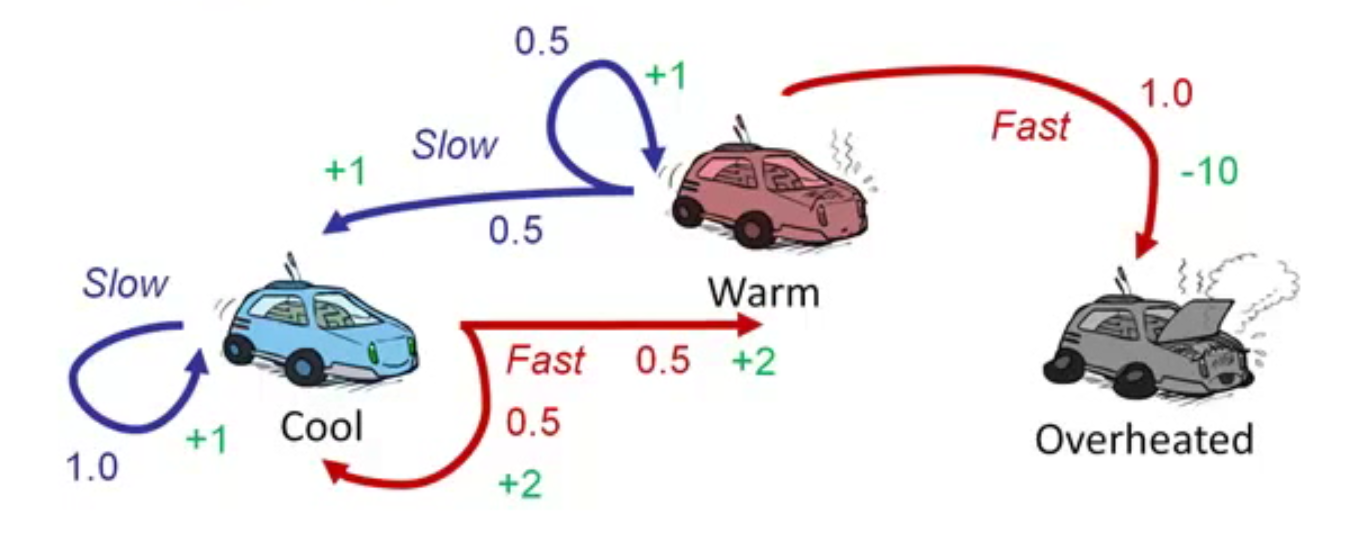
\includegraphics[width=0.7\linewidth]{Figures/rll6} 
\end{figure}
\end{enumerate}
\end{itemize}
\scriptsize [Pic: P. Abbeel]
\end{frame}

\begin{frame}\frametitle{Basic Problems}\small
\begin{itemize}
\item Markov Decision Problem (MDP): tuple $(S,A,P,\gamma)$ where $P$ is
\[
P(s_{t+1}=s', r_{t+1}=r' | s_t = s, a_t = a)
\]
\item Standard MDP problems:
\begin{enumerate}
\item  \high{Planning}: given complete Markov decision problem as input, compute policy with optimal expected return\\[1mm]
\item \high{Learning}: We don't know which states are good or what the actions do. We must try out the actions and states to learn what to do
\end{enumerate}
\end{itemize}
\vspace{28mm}
\scriptsize [P. Abbeel]
\end{frame}

\begin{frame}\frametitle{Example of Standard MDP Problem}\small
\begin{center}
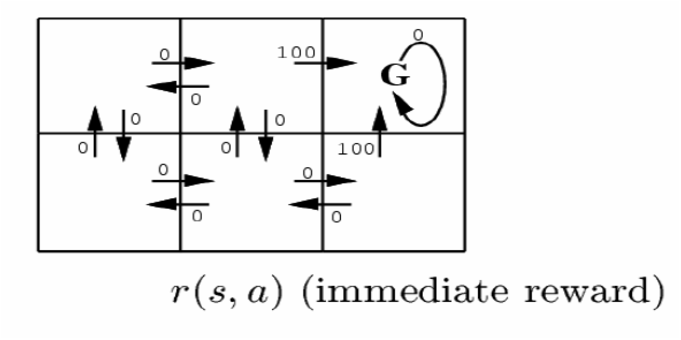
\includegraphics[width=0.54\linewidth]{Figures/tic_tac_rl} 
\end{center}
\begin{enumerate}
\item  \high{Planning}: given complete Markov decision problem as input, compute policy with optimal expected return
\item \high{Learning}: Only have access to experience in the MDP, learn a near-optimal strategy
\end{enumerate}
%We will focus on learning, but discuss planning along the way
\end{frame}

\begin{frame}\frametitle{Example of Standard MDP Problem}\small
\begin{center}
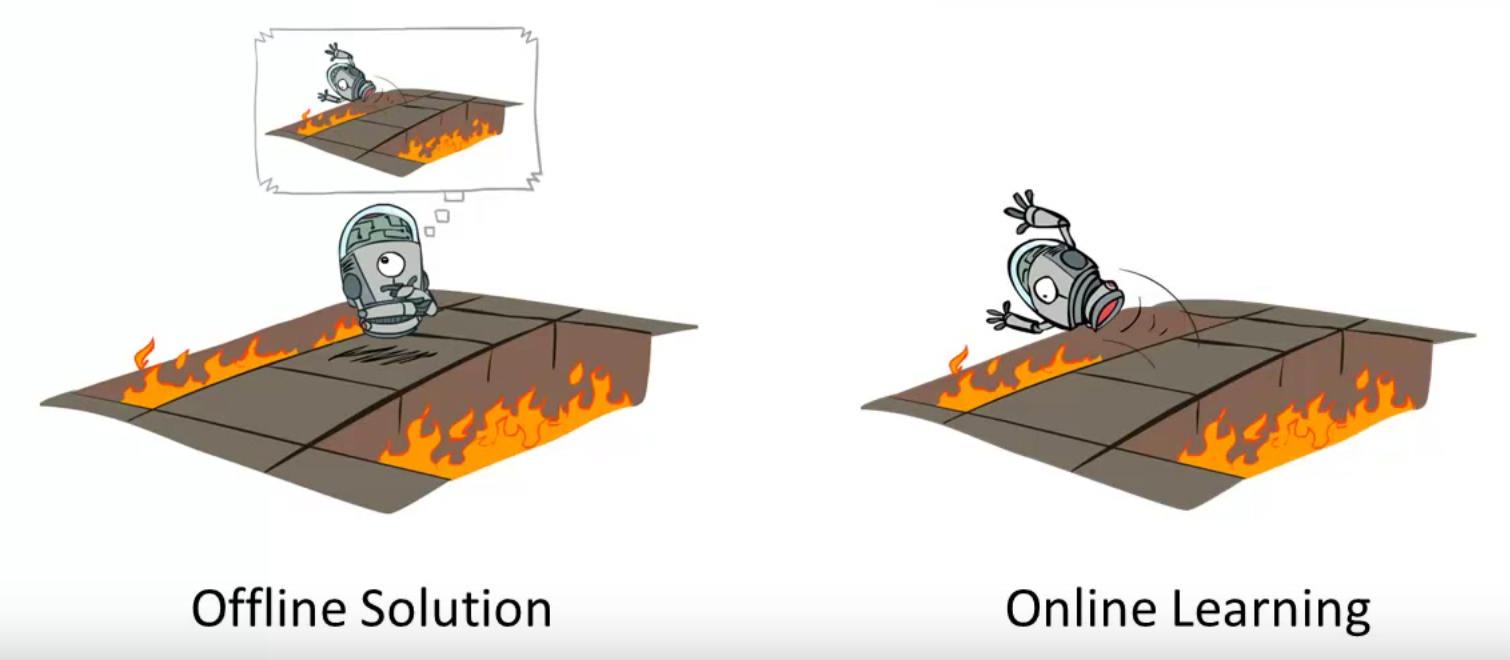
\includegraphics[width=0.785\linewidth,trim=0 50 0 0,clip]{Figures/rll4} 
\end{center}
\begin{enumerate}
\item  \high{Planning}: given complete Markov decision problem as input, compute policy with optimal expected return
\item \high{Learning}: Only have access to experience in the MDP, learn a near-optimal strategy
\end{enumerate}
We will focus on learning, but discuss planning along the way
\end{frame}

\begin{frame}\frametitle{Exploration vs. Exploitation}\small
\begin{itemize}
\item If we knew how the world works (embodied in $P$), then the policy should be deterministic 
\begin{itemize}
\onslide<2->\item  just select optimal action in each state
\end{itemize}
\onslide<3->\item Reinforcement learning is like trial-and-error learning
\onslide<4->\item The agent should discover a good policy from its experiences of the environment
\onslide<4->\item Without losing too much reward along the way

\onslide<5->\item Since we do not have complete knowledge of the world, taking what appears to be the optimal action may prevent us from finding better states/actions
\onslide<6->\item Interesting trade-off: 
\begin{itemize}
\item immediate reward (\high{exploitation}) vs. gaining knowledge that might enable higher future reward (\high{exploration})
\end{itemize}
\end{itemize}
\end{frame}

\begin{frame}\frametitle{Examples}\small
\begin{itemize}
\item Restaurant Selection
\begin{itemize}
\item \high{Exploitation}: Go to your favourite restaurant
\item \high{Exploration}: Try a new restaurant
\end{itemize}
\item Online Banner Advertisements
\begin{itemize}
\item \high{Exploitation}: Show the most successful advert
\item \high{Exploration}: Show a different advert
\end{itemize}
\item Oil Drilling
\begin{itemize}
\item \high{Exploitation}: Drill at the best known location
\item \high{Exploration}: Drill at a new location
\end{itemize}
\item Game Playing
\begin{itemize}
\item \high{Exploitation}: Play the move you believe is best
\item \high{Exploration}: Play an experimental move
\end{itemize}
\end{itemize}
\vspace{1mm}
\scriptsize [Slide credit: D. Silver]
\end{frame}

\begin{frame}\frametitle{Value function}\small
\begin{itemize}
\item The value function $V^\pi(s)$ assigns each state the expected reward 
\[
V^\pi(s)=\underset{a_{t},a_{t+i},s_{t+i}}{\mathbb{E}}\left[\sum_{i=1}^\infty\gamma^{i} r_{t+i} |s_t=s\right]
\]
\onslide<2->\item Usually not informative enough to make decisions.
\onslide<3->\item The $Q$-value $Q^{\pi}(s,a)$ is the expected reward of taking action $a$ in state $s$ and then continuing according to $\pi$.
\[
Q^\pi(s,a)=\underset{a_{t+i},s_{t+i}}{\mathbb{E}}\left[\sum_{i=1}^\infty\gamma^{i} r_{t+i} |s_t=s,a_t=a\right]
\]
\end{itemize}
\end{frame}

\begin{frame}\frametitle{Bellman equations}\small
\begin{itemize}
    \item The foundation of many RL algorithms
    {\footnotesize
    \begin{align*}\footnotesize
    V^\pi(s)&=\underset{a_{t},a_{t+i},s_{t+i}}{\mathbb{E}}\left[\sum_{i=1}^\infty\gamma^{i} r_{t+i} |s_t=s\right] \\
    &=\underset{a_{t}}{\mathbb{E}}\left[r_{t+1} |s_t=s\right]  +\gamma \underset{a_{t},a_{t+i},s_{t+i}}{\mathbb{E}}\left[\sum_{i=1}^\infty\gamma^{i} r_{t+i+1} |s_t=s\right] \\
    & = \underset{a_{t}}{\mathbb{E}}\left[r_{t+1} |s_t=s\right] +\gamma \underset{s_{t+1}}{\mathbb{E}}\left[V^{\pi}(s_{t+1})|s_t=s\right] \\
    & = \sum_{a,r}P^{\pi}(a|s_t)p(r|a,s_t)\cdot r+\gamma \sum_{a,s'}P^{\pi}(a|s_t)p(s'|a,s_t)\cdot V^{\pi}(s')
    \end{align*}}
    \item Similar equation holds for $Q$
        {\footnotesize
        \begin{align*}\footnotesize
        &Q^\pi(s,a)=\underset{a_{t+i},s_{t+i}}{\mathbb{E}}\left[\sum_{i=1}^\infty\gamma^{i} r_{t+i} |s_t=s,a_t=a\right] \\
        & = \sum_{r}p(r|a,s_t)\cdot r+ \gamma\sum_{s'}p(s'|a,s_t)\cdot V^{\pi}(s') \\
        &=\sum_{r}p(r|a,s_t)\cdot r+ \gamma\sum_{a',s'}p(s'|a,s_t)p(a'|s')\cdot Q^{\pi}(s',a')
        \end{align*}}
\end{itemize}
\end{frame}

\begin{frame}\frametitle{Solving Bellman equations}\small
\begin{itemize}
    \item The Bellman equations are a set of linear equations with a unique solution.
    % \onslide<2->\item Can solve fast(er) because the linear mapping is a contractive mapping.
    \onslide<2->\item This lets you know the quality of each state/action under your policy - \high{policy evaluation}.
    \onslide<3->\item You can improve by picking $\pi'(s)=\max_a Q^{\pi}(s,a)$ - \high{policy improvement}.
    \onslide<4->\item Can show the iterative policy evaluation and improvement converges to the optimal policy - \high{policy iteration}.
    \onslide<5->\item Are we done? % \onslide<7-> Why isn't this enough?
    \onslide<6->
    \begin{itemize}
        \item Need to know the model. Usually isn't known.
        \item Number of states is usually huge (how many unique states does a chess game have?) 
    \end{itemize}
\end{itemize}
\end{frame}

\begin{frame}\frametitle{Optimal Bellman equations}\small
\begin{itemize}
    \item First step is understand the Bellman equation for the optimal policy $\pi^*$
    \onslide<2->\item Under this policy $V^*(s)=\max_a Q^*(s,a)$
        {\footnotesize
        \begin{align*}\footnotesize
        V^*(s)& = \max_a\left[\mathbb{E}\left[r_{t+1} |s_t=s,a_t=a\right] +\gamma \underset{s_{t+1}}{\mathbb{E}}\left[V^{*}(s_{t+1})|s_t=s,a_t=a\right]\right] \\
        &= \max_a\left[\sum_{r}p(r|a,s_t)\cdot r+\gamma \sum_{s'}p(s'|a,s_t)\cdot V^*(s')\right] \\
        Q^*(s,a)&=\mathbb{E}\left[r_{t+1} |s_t=s,a_t=a\right]+ \gamma\underset{s_{t+1}}{\mathbb{E}}\left[\max_{a'}Q^{*}(s_{t+1},a')|s_t=s,a_t=a\right] \\
        &= \sum_{r}p(r|a,s_t)\cdot r+\gamma \sum_{s'}p(s'|a,s_t)\cdot\max_{a'} Q^*(s',a')
        \end{align*}}
    \onslide<3-> \item Set on nonlinear equations.
    \onslide<4-> \item Same issues as before.
\end{itemize}
\end{frame}


\begin{frame}\frametitle{Q-learning intuition}\small
\begin{itemize}
    \item Q-learning is a simple algorithm to find the optimal policy without knowing the model.
        \onslide<2->\item $Q^*$ is the unique solution to the optimal Bellman equation.
    \[
    Q^*(s,a)=\mathbb{E}\left[r_{t+1} |s_t=s,a_t=a\right]+ \gamma\underset{s_{t+1}}{\mathbb{E}}\left[\max_{a'}Q^{*}(s_{t+1},a')|s_t=s,a_t=a\right]
    \]
    \onslide<3->\item We don't know the model and don't want to update all states simultaneously.
    \onslide<4->\item Solution - given sample $s_t,a_t,r_{t+1},s_{t+1}$ from the environment update your $Q$-values so they are closer to satisfying the bellman equation.
    \begin{itemize}
        \item \high{off-policy} method: Samples don't have to be from the optimal policy.
    \end{itemize} 
    \item Samples need to be diverse enough to see everything - exploration.
\end{itemize}
\end{frame}

\begin{frame}\frametitle{Exploration vs exploitation}\small
\begin{itemize}
    \item Given $Q$-value the best thing we can do (given our limited knowledge) is to take $a=\arg\max_{a'}Q(s,a')$ - \high{exploitation}
    \onslide<2->\item How do we balance exploration with exploitation?
    \onslide<3->\item Simplest solution: $\epsilon$-greedy. 
    \begin{itemize}
        \item With probability $1-\epsilon$ pick $a=\arg\max_{a'}Q(s,a')$ (i.e. greedy)
        \item With probability $\epsilon$ pick any other action uniformly.
    \end{itemize} 
    \onslide<4->\item Another idea - softmax using $Q$ values
    \begin{itemize}
        \item With probability $1-\epsilon$ pick $a=\arg\max_{a'}Q(s,a')$ (i.e. greedy)
        \item With probability $\epsilon$ pick any other action with probability $\propto\exp(\beta Q(s,a))$.
    \end{itemize} 
    \onslide<5->\item Other fancier solutions exist, many leading methods use simple $\epsilon$-greedy sampling.
\end{itemize}
\end{frame}


\begin{frame}\frametitle{Q-learning algorithm}\small
\vspace{-0.5cm}
\begin{figure}
     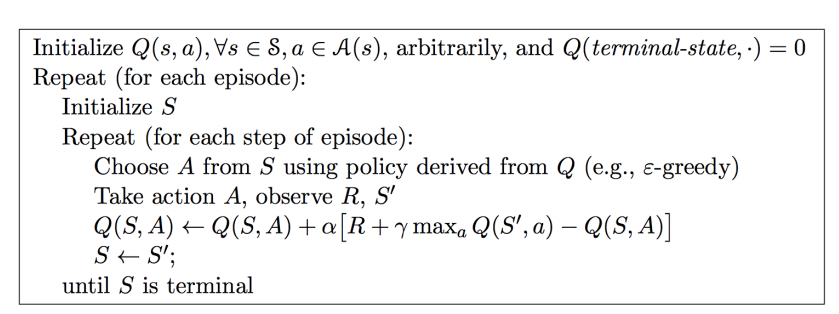
\includegraphics[width=0.9\linewidth]{Figures/Qalgo}
 \end{figure}
\vspace{-0.5cm}
\begin{itemize}
    \onslide<2->\item Can prove convergence to the optimal $Q^*$ under mild conditions.
    \onslide<3->\item Update is equivalent to gradient descent on loss $||R+\gamma\max_a Q(S',a)-Q(s,a)||^2$.
    \item At optimal Q, the loss is 0.
    % \onslide<4->\item Why $L_2$ loss? Optimal solution is the mean which is what we are looking for!
\end{itemize}
\end{frame}

\begin{frame}\frametitle{Bootstrapping}\small
\begin{itemize}
    \item Another way to think about Q-learning.
    \item $Q(s,a)$ is the expected reward, can use Monte-Carlo estimation.
    \onslide<2->\item Problem - you update only after the episode ends, can be very long (or infinite).
    \onslide<3->\item Q-learning solution - take only 1 step forward and estimate the future using our Q value - \high{bootstrapping}.
    \begin{itemize}
        \item "learn a guess from a guess"
    \end{itemize} 
    \onslide<4->\item Q-learning is just one algorithm in a family of algorithms that use this idea.
\end{itemize}
\end{frame}

\begin{frame}\frametitle{Function approximation}\small
\begin{itemize}
    \item Q-learning still scales badly with large state spaces, how many states does a chess game have? Need to save the full table!
    \onslide<2->\item Similar states, e.g. move all chess pieces two steps to the left, at treated as totally different.
    \onslide<3->\item Solution: Instead of $Q$ being a $S\times A$ table it is a parametrized function.
    \onslide<4-> \item Looking for function $\hat{Q}(s,a;\bw)\approx Q^*(s,a)$
    \begin{itemize}
        \onslide<5->\item Linear functions $Q(s,a;\bw)=\bw^T\phi(s,a)$.
        \item Neural network
    \end{itemize}
    \onslide<5->\item Hopefully can generalize to unseen states.
    \onslide<6->\item Problem: Each change to parameters changes all states/actions - can lead to instability.
    \onslide<7->\item For non-linear Q-learning can diverge.
\end{itemize}
\end{frame}


\begin{frame}\frametitle{Deep Q-learning}\small
\begin{itemize}
    \item We have a function approximator $Q(s,a;\theta)$, standard is neural net but doesn't have to be.
    \onslide<2->\item What is the objective that we are optimizing?
    \onslide<3->\item  We want to minimize $\mathbb{E}_{\rho}[||R+\gamma\max_{a'} Q(S',a')-Q(s,a)||^2]$
    \begin{itemize}
        \item $\rho$ is a distribution over states, depends on $\theta$!
    \end{itemize}
    \onslide<4->\item Two terms depend on $Q$, don't want to take gradients w.r. to $\gamma\max_aQ(S',a)$
    \onslide<5->\item We want to correct our previous estimation given the new information.
            \vspace{-0.2cm}
    \begin{figure}
        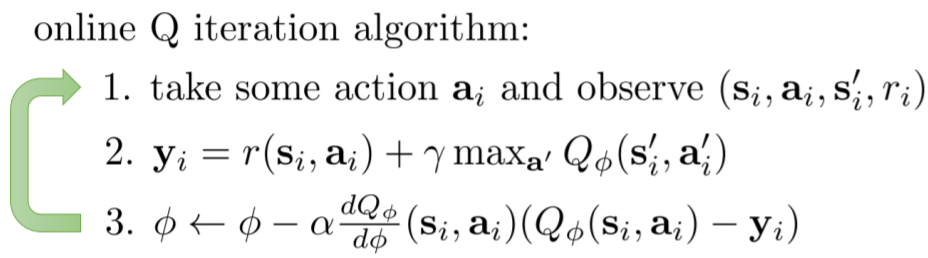
\includegraphics[width=0.85\linewidth]{Figures/Qalgo2}
        \vspace{-0.4cm}
        \caption{Take from:rll.berkeley.edu/deeprlcourse}
    \end{figure}
        \vspace{-0.5cm}
    \onslide<5->\item This simple approach doesn't work well as is.
\end{itemize}
\end{frame}

\begin{frame}\frametitle{Issues and solutions}\small
\begin{itemize}
    \item \high{Problem}: data in the minibatch is highly correlated
    \begin{itemize}
        \item Consecutive samples are from the same eposide and probably similar states.
        \item Solution: \high{Replay memory}.
        \item You store a large memory buffer of previous $(s,a,r,s')$ (notice this is all you need for Q-learning) and sample from it to get diverse minibatch.
    \end{itemize}
    \item \high{Problem}: The data distribution keeps changing
\begin{itemize}
    \item Since we aren't optimizing $y_i$ its like solving a different (but related) least squares each iteration.
    \item We can stabilize by fixing a \high{target network} for a few iterations 
\end{itemize}
\end{itemize}
    \begin{figure}
    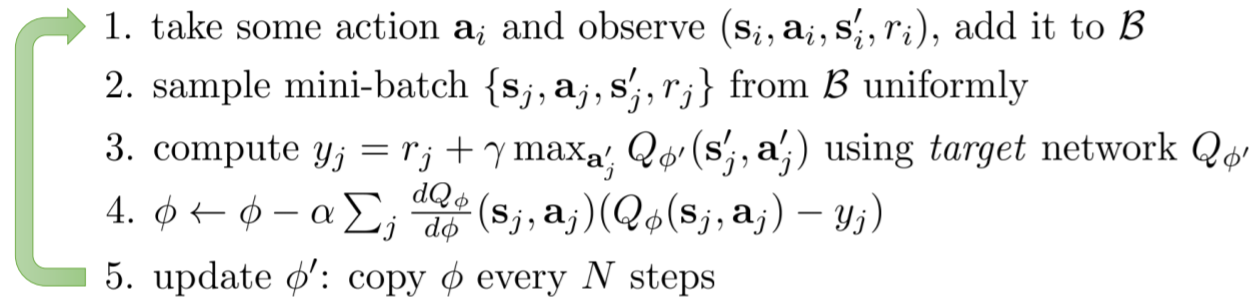
\includegraphics[width=0.75\linewidth]{Figures/DQN}
    \vspace{-0.4cm}
    \caption{Take from:rll.berkeley.edu/deeprlcourse}
\end{figure}
\end{frame}

\begin{frame}\frametitle{Example: DQN on atari}\small
\begin{itemize}
    \item Trained a NN from scratch on atari games 

\begin{figure}
    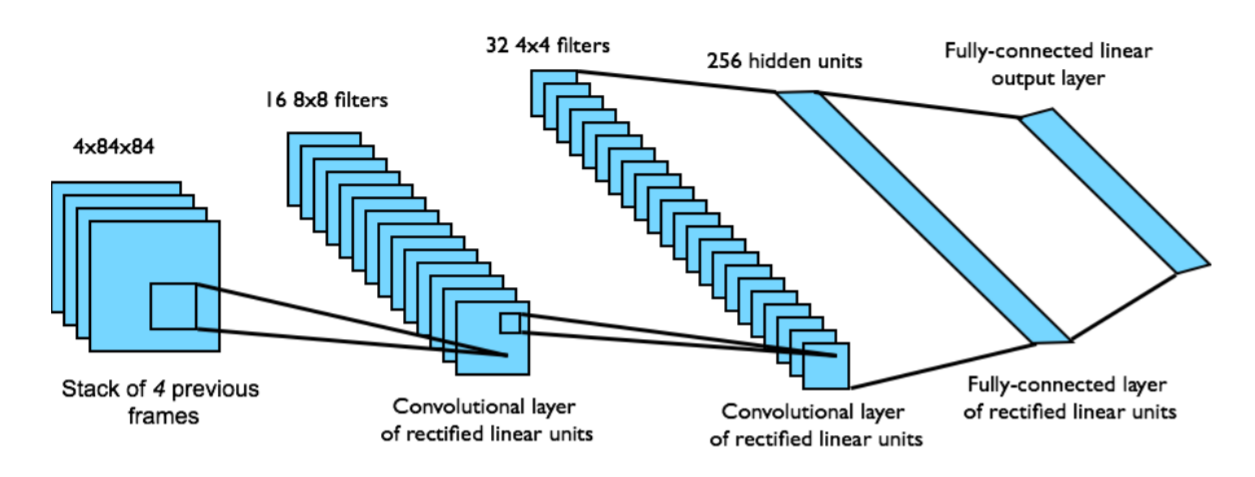
\includegraphics[width=0.75\linewidth]{Figures/DQN_arc}
\end{figure}
\onslide<2->\item Ablation study
\begin{figure}
    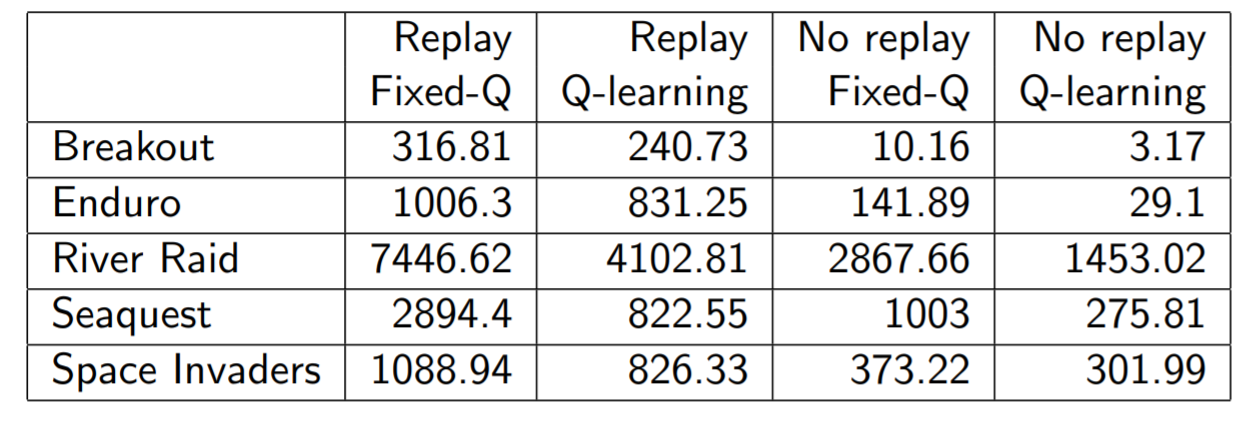
\includegraphics[width=0.75\linewidth]{Figures/ablation}
\end{figure}
\end{itemize}
\end{frame}


\begin{frame}\frametitle{RL recap}\small

\begin{itemize}
    \item Learning from experience not from labeled examples.
    \onslide<2->\item Why is RL hard?
    \begin{itemize}
        \onslide<3->\item Limited feedback.
        \onslide<4->\item Delayed rewards.
        \onslide<5->\item Your model effect what you
         see.
        \onslide<6->\item Huge state space.
    \end{itemize}
    \onslide<7-> \item Usually solved by learning the value function or optimizing the policy (not covered)
    % \onslide<8-> \item Model based method but less successful at the moment.
    \onslide<9-> \item How do you define the rewards? Can be tricky.
    \begin{itemize}
        \item Bad rewards can lead to \high{reward hacking}
        \url{https://www.youtube.com/watch?v=tlOIHko8ySg}
    \end{itemize}
\end{itemize}
\end{frame}

\begin{frame}\frametitle{Q-Learning recap}
\begin{itemize}
    \item Try to find $Q$ that satisfies the optimal Bellman conditions
    \onslide<2->\item \high{Off-policy} algorithm - Doesn't have to follow a greedy policy to evaluate it.
    \onslide<3->\item \high{Model free} algorithm - Doesn't have any model for instantaneous reward or dynamics.
    \onslide<4->\item Learns a seperate value for each $s,a$ pair - doesn't scale up to huge state spaces.
    \onslide<5->\item Can scale using a function approximation
    \begin{itemize}
        \item No more theoretical guarantees.
        \item Can diverge. 
        \item Some simple tricks help a lot.
    \end{itemize}
\end{itemize}
\end{frame}
\end{document}